\documentclass[a4paper,12pt]{article}\usepackage[]{graphicx}\usepackage[]{color}
%% maxwidth is the original width if it is less than linewidth
%% otherwise use linewidth (to make sure the graphics do not exceed the margin)
\makeatletter
\def\maxwidth{ %
  \ifdim\Gin@nat@width>\linewidth
    \linewidth
  \else
    \Gin@nat@width
  \fi
}
\makeatother

\definecolor{fgcolor}{rgb}{0.345, 0.345, 0.345}
\newcommand{\hlnum}[1]{\textcolor[rgb]{0.686,0.059,0.569}{#1}}%
\newcommand{\hlstr}[1]{\textcolor[rgb]{0.192,0.494,0.8}{#1}}%
\newcommand{\hlcom}[1]{\textcolor[rgb]{0.678,0.584,0.686}{\textit{#1}}}%
\newcommand{\hlopt}[1]{\textcolor[rgb]{0,0,0}{#1}}%
\newcommand{\hlstd}[1]{\textcolor[rgb]{0.345,0.345,0.345}{#1}}%
\newcommand{\hlkwa}[1]{\textcolor[rgb]{0.161,0.373,0.58}{\textbf{#1}}}%
\newcommand{\hlkwb}[1]{\textcolor[rgb]{0.69,0.353,0.396}{#1}}%
\newcommand{\hlkwc}[1]{\textcolor[rgb]{0.333,0.667,0.333}{#1}}%
\newcommand{\hlkwd}[1]{\textcolor[rgb]{0.737,0.353,0.396}{\textbf{#1}}}%

\usepackage{framed}
\makeatletter
\newenvironment{kframe}{%
 \def\at@end@of@kframe{}%
 \ifinner\ifhmode%
  \def\at@end@of@kframe{\end{minipage}}%
  \begin{minipage}{\columnwidth}%
 \fi\fi%
 \def\FrameCommand##1{\hskip\@totalleftmargin \hskip-\fboxsep
 \colorbox{shadecolor}{##1}\hskip-\fboxsep
     % There is no \\@totalrightmargin, so:
     \hskip-\linewidth \hskip-\@totalleftmargin \hskip\columnwidth}%
 \MakeFramed {\advance\hsize-\width
   \@totalleftmargin\z@ \linewidth\hsize
   \@setminipage}}%
 {\par\unskip\endMakeFramed%
 \at@end@of@kframe}
\makeatother

\definecolor{shadecolor}{rgb}{.97, .97, .97}
\definecolor{messagecolor}{rgb}{0, 0, 0}
\definecolor{warningcolor}{rgb}{1, 0, 1}
\definecolor{errorcolor}{rgb}{1, 0, 0}
\newenvironment{knitrout}{}{} % an empty environment to be redefined in TeX

\usepackage{alltt}
\usepackage[margin=2cm]{geometry}
\usepackage{placeins}

\title{Exp 2 of 4}
\IfFileExists{upquote.sty}{\usepackage{upquote}}{}
\begin{document}



\maketitle
\tableofcontents
\clearpage














\clearpage
\section{Get the data}

\begin{knitrout}\scriptsize
\definecolor{shadecolor}{rgb}{0.969, 0.969, 0.969}\color{fgcolor}\begin{kframe}
\begin{alltt}
\hlcom{# if the file data_processed.Rda already exists then load it, else do data wrangling}
\hlkwa{if} \hlstd{(}\hlkwd{file.exists}\hlstd{(}\hlstr{"data_processed.Rda"}\hlstd{)) \{}
    \hlkwd{load}\hlstd{(}\hlstr{"data_processed.Rda"}\hlstd{)}
\hlstd{\}} \hlkwa{else} \hlstd{\{}
    \hlcom{# declare local variables}
    \hlstd{number_of_valid_subjects} \hlkwb{<-} \hlnum{30}  \hlcom{# = 30}
    \hlstd{number_of_rows} \hlkwb{<-} \hlnum{7680}  \hlcom{# 7680}
    \hlstd{number_of_trials_per_subject} \hlkwb{<-} \hlstd{number_of_rows}\hlopt{/}\hlstd{number_of_valid_subjects}  \hlcom{# = 256}
    \hlcom{# call functions}
    \hlstd{dat} \hlkwb{<-} \hlkwd{gatherData}\hlstd{(number_of_valid_subjects)}  \hlcom{# = 30}
    \hlstd{dat} \hlkwb{<-} \hlkwd{classifyResponses}\hlstd{(dat)}  \hlcom{# classify the response as expected, near, or far}
    \hlstd{dat} \hlkwb{<-} \hlkwd{processData}\hlstd{(dat)}  \hlcom{# remove impossible trials and re-do previous rt measures}
    \hlstd{dd} \hlkwb{<-} \hlkwd{postProcessData}\hlstd{(dat)}
\hlstd{\}}  \hlcom{# end else do data wrangling}
\end{alltt}
\end{kframe}
\end{knitrout}

\begin{knitrout}\scriptsize
\definecolor{shadecolor}{rgb}{0.969, 0.969, 0.969}\color{fgcolor}\begin{kframe}
\begin{alltt}
\hlkwd{names}\hlstd{(dd)}
\end{alltt}
\begin{verbatim}
 [1] "id"                "Subject"           "Trial"             "Condition"        
 [5] "Order"             "Quantity"          "Vagueness"         "Number"           
 [9] "Item"              "discriminability"  "c_Trl"             "s_Trl"            
[13] "c_Itm"             "c_Vag"             "c_Num"             "f_Cnd"            
[17] "c_Ord"             "c_Qty"             "RT"                "RT_log"           
[21] "RT_raw"            "RTprev"            "RTprev_log"        "RTprev_raw"       
[25] "Exp_Num"           "Bline_Num"         "Extr_Num"          "Exp_side"         
[29] "Bline_side"        "Extr_side"         "response_num"      "response_side"    
[33] "response_category" "Left"              "Mid"               "Right"            
[37] "Instruction"       "nchar_instr"      
\end{verbatim}
\end{kframe}
\end{knitrout}

\begin{knitrout}\scriptsize
\definecolor{shadecolor}{rgb}{0.969, 0.969, 0.969}\color{fgcolor}\begin{kframe}
\begin{alltt}
\hlkwd{head}\hlstd{(dd)}
\end{alltt}
\begin{verbatim}
        id Subject Trial Condition Order Quantity Vagueness  Number     Item discriminability
1 s01:t001     s01     1         2  RtoL    Small     Crisp Numeric 06:15:24        0.4875000
2 s01:t002     s01     2         1  LtoR    Large     Vague Numeric 16:25:34        0.3123529
3 s01:t003     s01     3         4  LtoR    Small     Crisp  Verbal 26:35:44        0.2308442
4 s01:t004     s01     4         1  RtoL    Large     Vague Numeric 36:45:54        0.1833333
5 s01:t005     s01     5         1  RtoL    Small     Vague Numeric 06:15:24        0.4875000
6 s01:t006     s01     6         3  LtoR    Large     Vague  Verbal 16:25:34        0.3123529
   c_Trl     s_Trl c_Itm c_Vag c_Num f_Cnd c_Ord c_Qty   RT   RT_log RT_raw RTprev RTprev_log
1 -127.5 -1.725186 -0.75  -0.5  -0.5 Cr:Nm   0.5  -0.5 1517 7.324490   1517   1517   7.324490
2 -126.5 -1.711655 -0.25   0.5  -0.5 Vg:Nm  -0.5   0.5 1920 7.560080   1920   1517   7.324490
3 -125.5 -1.698124  0.25  -0.5   0.5 Cr:Vb  -0.5  -0.5 2346 7.760467   2346   1920   7.560080
4 -124.5 -1.684593  0.75   0.5  -0.5 Vg:Nm   0.5   0.5 1773 7.480428   1773   2346   7.760467
5 -123.5 -1.671062 -0.75   0.5  -0.5 Vg:Nm   0.5  -0.5 2556 7.846199   2556   1773   7.480428
6 -122.5 -1.657531 -0.25   0.5   0.5 Vg:Vb  -0.5   0.5 2043 7.622175   2043   2556   7.846199
  RTprev_raw Exp_Num Bline_Num Extr_Num Exp_side Bline_side Extr_side response_num response_side
1       1517       6        15       24    right        mid      left            6         right
2       1517      34        25       16    right        mid      left           25           mid
3       1920      26        35       44     left        mid     right           26          left
4       2346      54        45       36     left        mid     right           45           mid
5       1773       6        15       24    right        mid      left            6         right
6       2556      34        25       16    right        mid      left           34         right
  response_category Left Mid Right                            Instruction nchar_instr
1          expected   24  15     6          Choose the square with 6 dots          29
2        borderline   16  25    34     Choose a square with about 30 dots          34
3          expected   26  35    44 Choose the square with the fewest dots          38
4        borderline   54  45    36     Choose a square with about 50 dots          34
5          expected   24  15     6     Choose a square with about 10 dots          34
6          expected   16  25    34         Choose a square with many dots          30
\end{verbatim}
\end{kframe}
\end{knitrout}

\begin{knitrout}\scriptsize
\definecolor{shadecolor}{rgb}{0.969, 0.969, 0.969}\color{fgcolor}\begin{kframe}
\begin{alltt}
\hlkwd{summary}\hlstd{(dd)}
\end{alltt}
\begin{verbatim}
        id          Subject         Trial         Condition    Order       Quantity    Vagueness   
 s01:t001:   1   s01    : 256   Min.   :  1.0   Min.   :1.0   LtoR:3838   Small:3840   Crisp:3840  
 s01:t002:   1   s02    : 256   1st Qu.: 65.0   1st Qu.:2.0   RtoL:3839   Large:3837   Vague:3837  
 s01:t003:   1   s03    : 256   Median :129.0   Median :3.0                                        
 s01:t004:   1   s04    : 256   Mean   :128.5   Mean   :2.5                                        
 s01:t005:   1   s05    : 256   3rd Qu.:193.0   3rd Qu.:4.0                                        
 s01:t006:   1   s06    : 256   Max.   :256.0   Max.   :4.0                                        
 (Other) :7671   (Other):6141                                                                      
     Number           Item      discriminability     c_Trl                s_Trl           
 Numeric:3838   06:15:24:1919   Min.   :0.1833   Min.   :-127.50000   Min.   :-1.7251858  
 Verbal :3839   16:25:34:1919   1st Qu.:0.2308   1st Qu.: -63.50000   1st Qu.:-0.8592102  
                26:35:44:1920   Median :0.2308   Median :   0.50000   Median : 0.0067654  
                36:45:54:1919   Mean   :0.3035   Mean   :   0.02377   Mean   : 0.0003217  
                                3rd Qu.:0.3124   3rd Qu.:  64.50000   3rd Qu.: 0.8727411  
                                Max.   :0.4875   Max.   : 127.50000   Max.   : 1.7251858  
                                                                                          
     c_Itm               c_Vag                c_Num             f_Cnd          c_Ord          
 Min.   :-7.50e-01   Min.   :-0.5000000   Min.   :-5.00e-01   Vg:Nm:1918   Min.   :-5.00e-01  
 1st Qu.:-2.50e-01   1st Qu.:-0.5000000   1st Qu.:-5.00e-01   Cr:Nm:1920   1st Qu.:-5.00e-01  
 Median : 2.50e-01   Median :-0.5000000   Median : 5.00e-01   Vg:Vb:1919   Median : 5.00e-01  
 Mean   : 3.26e-05   Mean   :-0.0001954   Mean   : 6.51e-05   Cr:Vb:1920   Mean   : 6.51e-05  
 3rd Qu.: 2.50e-01   3rd Qu.: 0.5000000   3rd Qu.: 5.00e-01                3rd Qu.: 5.00e-01  
 Max.   : 7.50e-01   Max.   : 0.5000000   Max.   : 5.00e-01                Max.   : 5.00e-01  
                                                                                              
     c_Qty                  RT            RT_log           RT_raw          RTprev     
 Min.   :-0.5000000   Min.   :  445   Min.   : 6.098   Min.   :  445   Min.   :  445  
 1st Qu.:-0.5000000   1st Qu.: 1240   1st Qu.: 7.123   1st Qu.: 1240   1st Qu.: 1240  
 Median :-0.5000000   Median : 1727   Median : 7.454   Median : 1727   Median : 1727  
 Mean   :-0.0001954   Mean   : 2840   Mean   : 7.595   Mean   : 2840   Mean   : 2835  
 3rd Qu.: 0.5000000   3rd Qu.: 2699   3rd Qu.: 7.901   3rd Qu.: 2699   3rd Qu.: 2697  
 Max.   : 0.5000000   Max.   :42685   Max.   :10.662   Max.   :42685   Max.   :42685  
                                                                                      
   RTprev_log       RTprev_raw       Exp_Num     Bline_Num     Extr_Num    Exp_side        
 Min.   : 6.098   Min.   :  445   Min.   : 6   Min.   :15   Min.   : 6   Length:7677       
 1st Qu.: 7.123   1st Qu.: 1240   1st Qu.:16   1st Qu.:25   1st Qu.:24   Class :character  
 Median : 7.454   Median : 1727   Median :26   Median :35   Median :34   Mode  :character  
 Mean   : 7.594   Mean   : 2835   Mean   :30   Mean   :30   Mean   :30                     
 3rd Qu.: 7.900   3rd Qu.: 2697   3rd Qu.:36   3rd Qu.:35   3rd Qu.:44                     
 Max.   :10.662   Max.   :42685   Max.   :54   Max.   :45   Max.   :54                     
                                                                                           
  Bline_side         Extr_side          response_num   response_side  response_category
 Length:7677        Length:7677        Min.   : 6.00   left :3215    borderline:1274   
 Class :character   Class :character   1st Qu.:24.00   mid  :1274    expected  :6108   
 Mode  :character   Mode  :character   Median :34.00   right:3188    extreme   : 295   
                                       Mean   :30.87                                   
                                       3rd Qu.:44.00                                   
                                       Max.   :54.00                                   
                                                                                       
      Left         Mid         Right                                    Instruction  
 Min.   : 6   Min.   :15   Min.   : 6   Choose a square with few dots         : 960  
 1st Qu.:24   1st Qu.:25   1st Qu.:24   Choose the square with the fewest dots: 960  
 Median :34   Median :35   Median :26   Choose the square with the most dots  : 960  
 Mean   :30   Mean   :30   Mean   :30   Choose a square with many dots        : 959  
 3rd Qu.:44   3rd Qu.:35   3rd Qu.:36   Choose a square with about 30 dots    : 480  
 Max.   :54   Max.   :45   Max.   :54   Choose a square with about 40 dots    : 480  
                                        (Other)                               :2878  
  nchar_instr   
 Min.   :29.00  
 1st Qu.:30.00  
 Median :30.00  
 Mean   :32.59  
 3rd Qu.:36.00  
 Max.   :38.00  
                
\end{verbatim}
\end{kframe}
\end{knitrout}

\begin{knitrout}\scriptsize
\definecolor{shadecolor}{rgb}{0.969, 0.969, 0.969}\color{fgcolor}\begin{kframe}
\begin{alltt}
\hlkwd{str}\hlstd{(dd)}
\end{alltt}
\begin{verbatim}
'data.frame':	7677 obs. of  38 variables:
 $ id               : Factor w/ 7680 levels "s01:t001","s01:t002",..: 1 2 3 4 5 6 7 8 9 10 ...
 $ Subject          : Factor w/ 30 levels "s01","s02","s03",..: 1 1 1 1 1 1 1 1 1 1 ...
 $ Trial            : int  1 2 3 4 5 6 7 8 9 10 ...
 $ Condition        : int  2 1 4 1 1 3 3 4 4 2 ...
 $ Order            : Factor w/ 2 levels "LtoR","RtoL": 2 1 1 2 2 1 2 2 1 2 ...
 $ Quantity         : Factor w/ 2 levels "Small","Large": 1 2 1 2 1 2 1 1 2 2 ...
 $ Vagueness        : Factor w/ 2 levels "Crisp","Vague": 1 2 1 2 2 2 2 1 1 1 ...
 $ Number           : Factor w/ 2 levels "Numeric","Verbal": 1 1 2 1 1 2 2 2 2 1 ...
 $ Item             : Factor w/ 4 levels "06:15:24","16:25:34",..: 1 2 3 4 1 2 3 4 1 2 ...
 $ discriminability : num  0.487 0.312 0.231 0.183 0.487 ...
 $ c_Trl            : num  -128 -126 -126 -124 -124 ...
 $ s_Trl            : num  -1.73 -1.71 -1.7 -1.68 -1.67 ...
 $ c_Itm            : num  -0.75 -0.25 0.25 0.75 -0.75 -0.25 0.25 0.75 -0.75 -0.25 ...
 $ c_Vag            : num  -0.5 0.5 -0.5 0.5 0.5 0.5 0.5 -0.5 -0.5 -0.5 ...
 $ c_Num            : num  -0.5 -0.5 0.5 -0.5 -0.5 0.5 0.5 0.5 0.5 -0.5 ...
 $ f_Cnd            : Factor w/ 4 levels "Vg:Nm","Cr:Nm",..: 2 1 4 1 1 3 3 4 4 2 ...
 $ c_Ord            : num  0.5 -0.5 -0.5 0.5 0.5 -0.5 0.5 0.5 -0.5 0.5 ...
 $ c_Qty            : num  -0.5 0.5 -0.5 0.5 -0.5 0.5 -0.5 -0.5 0.5 0.5 ...
 $ RT               : int  1517 1920 2346 1773 2556 2043 2384 3078 1760 2218 ...
 $ RT_log           : num  7.32 7.56 7.76 7.48 7.85 ...
 $ RT_raw           : int  1517 1920 2346 1773 2556 2043 2384 3078 1760 2218 ...
 $ RTprev           : int  1517 1517 1920 2346 1773 2556 2043 2384 3078 1760 ...
 $ RTprev_log       : num  7.32 7.32 7.56 7.76 7.48 ...
 $ RTprev_raw       : int  1517 1517 1920 2346 1773 2556 2043 2384 3078 1760 ...
 $ Exp_Num          : num  6 34 26 54 6 34 26 36 24 34 ...
 $ Bline_Num        : num  15 25 35 45 15 25 35 45 15 25 ...
 $ Extr_Num         : num  24 16 44 36 24 16 44 54 6 16 ...
 $ Exp_side         : chr  "right" "right" "left" "left" ...
 $ Bline_side       : chr  "mid" "mid" "mid" "mid" ...
 $ Extr_side        : chr  "left" "left" "right" "right" ...
 $ response_num     : int  6 25 26 45 6 34 26 36 24 25 ...
 $ response_side    : Factor w/ 3 levels "left","mid","right": 3 2 1 2 3 3 3 3 3 2 ...
 $ response_category: Factor w/ 3 levels "borderline","expected",..: 2 1 2 1 2 2 2 2 2 1 ...
 $ Left             : int  24 16 26 54 24 16 44 54 6 34 ...
 $ Mid              : int  15 25 35 45 15 25 35 45 15 25 ...
 $ Right            : int  6 34 44 36 6 34 26 36 24 16 ...
 $ Instruction      : Factor w/ 17 levels "Choose a square with about 10 dots",..: 15 3 16 5 1 7 6 16 17 11 ...
 $ nchar_instr      : int  29 34 38 34 34 30 29 38 36 30 ...
\end{verbatim}
\end{kframe}
\end{knitrout}

\clearpage
\section{Plots}
\clearpage
\subsection{Discriminability}

\begin{knitrout}\scriptsize
\definecolor{shadecolor}{rgb}{0.969, 0.969, 0.969}\color{fgcolor}\begin{figure}[hbtp]

{\centering 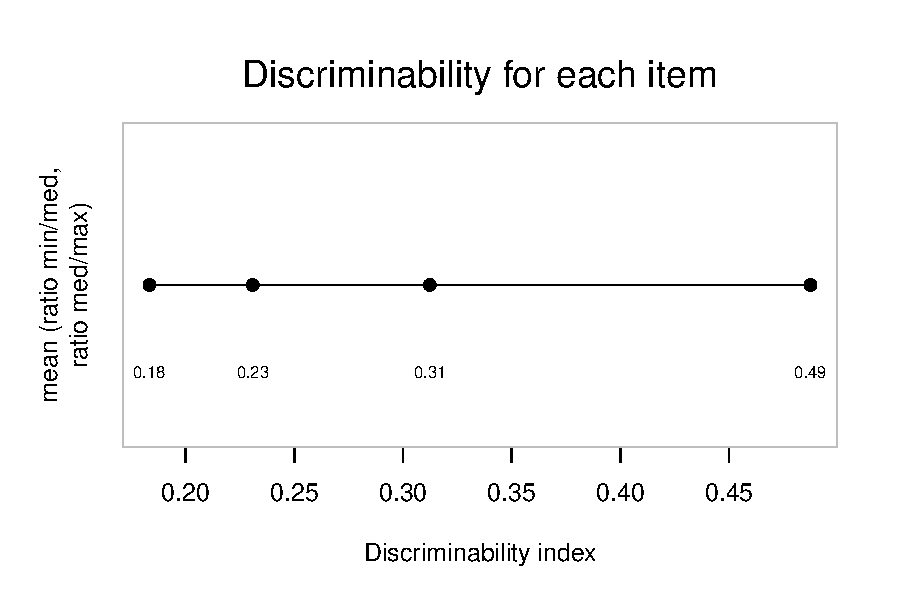
\includegraphics[width=\maxwidth]{figure/graphics-showCompression-1} 

}

\caption[Ratios for different numbers of dots in the arrays]{Ratios for different numbers of dots in the arrays: smaller values are more discriminable. Blue is for the ratio between the smallest number in the array and the largest number in an array. Red is for the mean of two ratios, one for the smallest number to the middle number, the other for the middle number to the largest number in the array}\label{fig:showCompression}
\end{figure}


\end{knitrout}

\clearpage



\begin{knitrout}\scriptsize
\definecolor{shadecolor}{rgb}{0.969, 0.969, 0.969}\color{fgcolor}\begin{figure}[hbtp]

{\centering 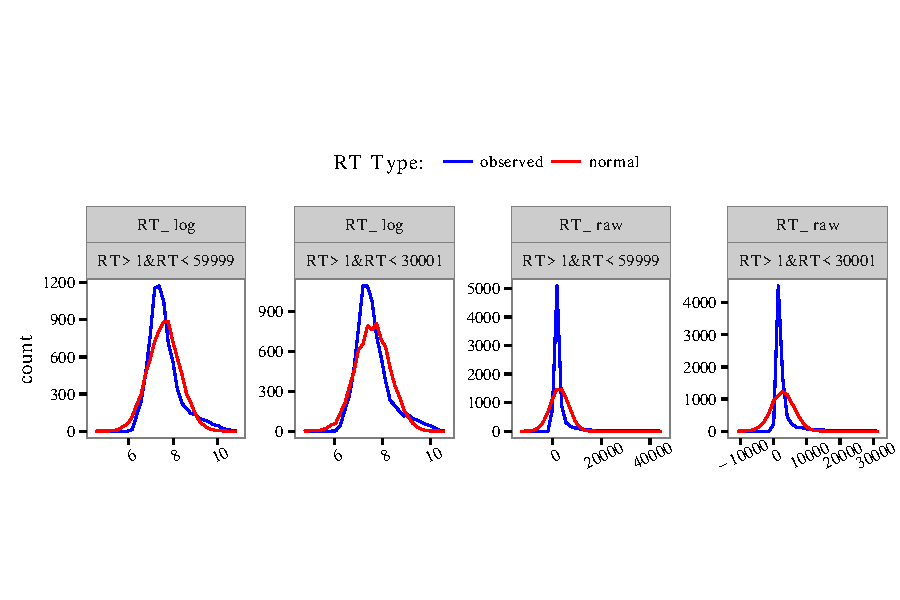
\includegraphics[width=\maxwidth]{figure/graphics-plotDistFreqPolys-1} 

}

\caption[Compare distributions of the various transformations of RT against random samples from normal distributions with the same mean and sd to see which transformations best approximate normal distributions]{Compare distributions of the various transformations of RT against random samples from normal distributions with the same mean and sd to see which transformations best approximate normal distributions}\label{fig:plotDistFreqPolys}
\end{figure}


\end{knitrout}

\clearpage

\begin{knitrout}\scriptsize
\definecolor{shadecolor}{rgb}{0.969, 0.969, 0.969}\color{fgcolor}\begin{figure}[hbtp]

{\centering 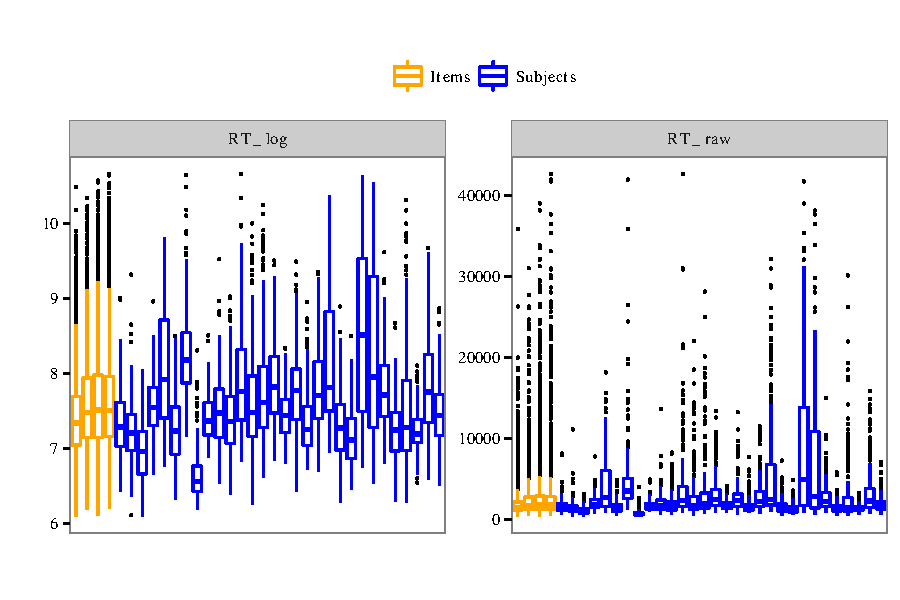
\includegraphics[width=\maxwidth]{figure/graphics-plotBoxPlots-1} 

}

\caption[Show how transformations of RT affect distribution of times, and how they affect which times are outliers]{Show how transformations of RT affect distribution of times, and how they affect which times are outliers.}\label{fig:plotBoxPlots}
\end{figure}


\end{knitrout}

\clearpage

\begin{knitrout}\scriptsize
\definecolor{shadecolor}{rgb}{0.969, 0.969, 0.969}\color{fgcolor}\begin{figure}[hbtp]

{\centering 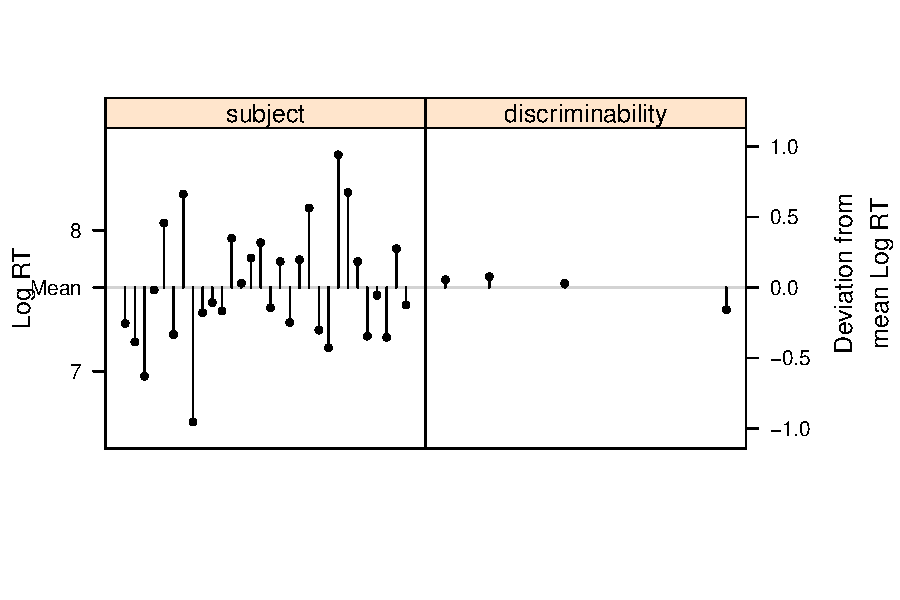
\includegraphics[width=\maxwidth]{figure/graphics-plotFastSlowRTs-1} 

}

\caption[Show how mean times for individual subjects and items vary with respect to the grand mean Log RT]{Show how mean times for individual subjects and items vary with respect to the grand mean Log RT.}\label{fig:plotFastSlowRTs}
\end{figure}


\end{knitrout}

\clearpage

\begin{knitrout}\scriptsize
\definecolor{shadecolor}{rgb}{0.969, 0.969, 0.969}\color{fgcolor}\begin{figure}[hbtp]

{\centering 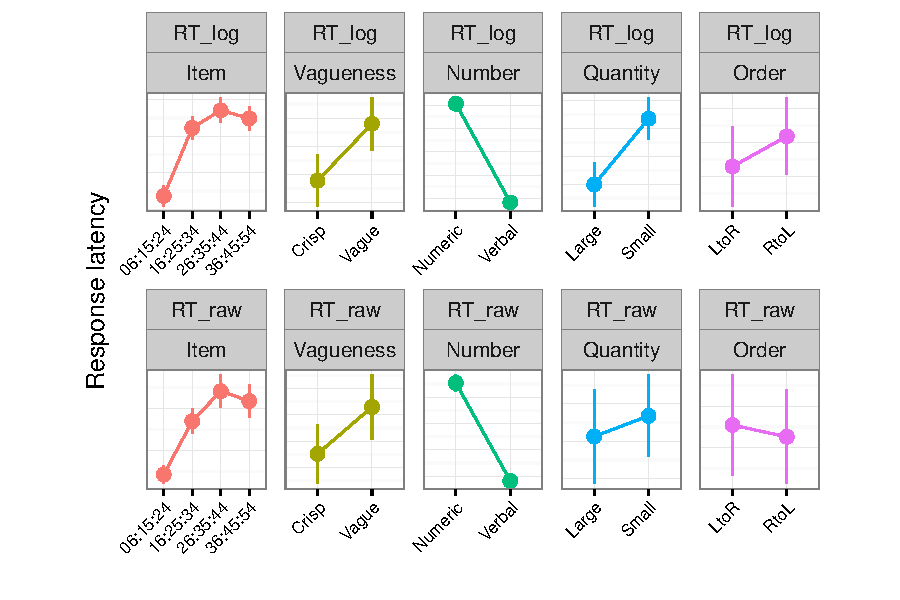
\includegraphics[width=\maxwidth]{figure/graphics-plotMainsa-1} 

}

\caption[Plot main effects on several transformations]{Plot main effects on several transformations}\label{fig:plotMainsa}
\end{figure}


\end{knitrout}

\clearpage

\begin{knitrout}\scriptsize
\definecolor{shadecolor}{rgb}{0.969, 0.969, 0.969}\color{fgcolor}\begin{figure}[hbtp]

{\centering 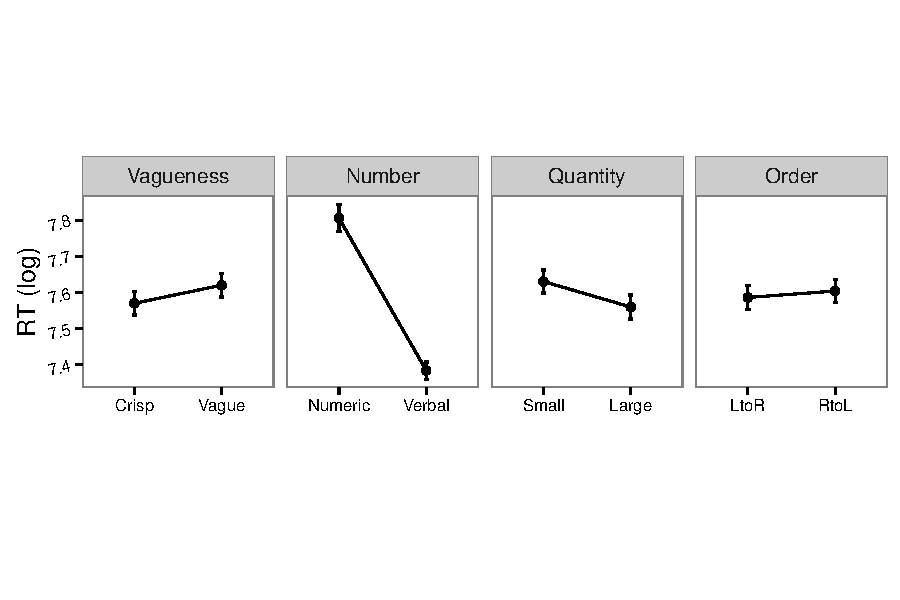
\includegraphics[width=\maxwidth]{figure/graphics-mainB-1} 

}

\caption[Just the main effects]{Just the main effects}\label{fig:mainB}
\end{figure}


\end{knitrout}

\clearpage

\begin{knitrout}\scriptsize
\definecolor{shadecolor}{rgb}{0.969, 0.969, 0.969}\color{fgcolor}\begin{figure}[hbtp]

{\centering 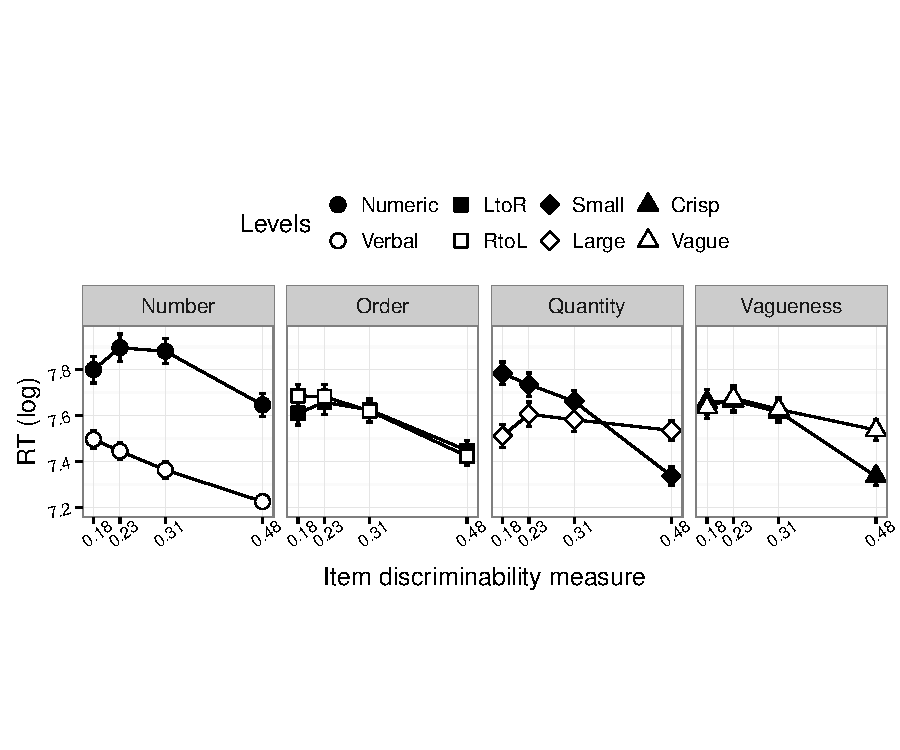
\includegraphics[width=\maxwidth]{figure/graphics-mainD-1} 

}

\caption[Main effects over item ratios]{Main effects over item ratios}\label{fig:mainD}
\end{figure}


\end{knitrout}

\clearpage

\begin{knitrout}\scriptsize
\definecolor{shadecolor}{rgb}{0.969, 0.969, 0.969}\color{fgcolor}\begin{figure}[hbtp]

{\centering 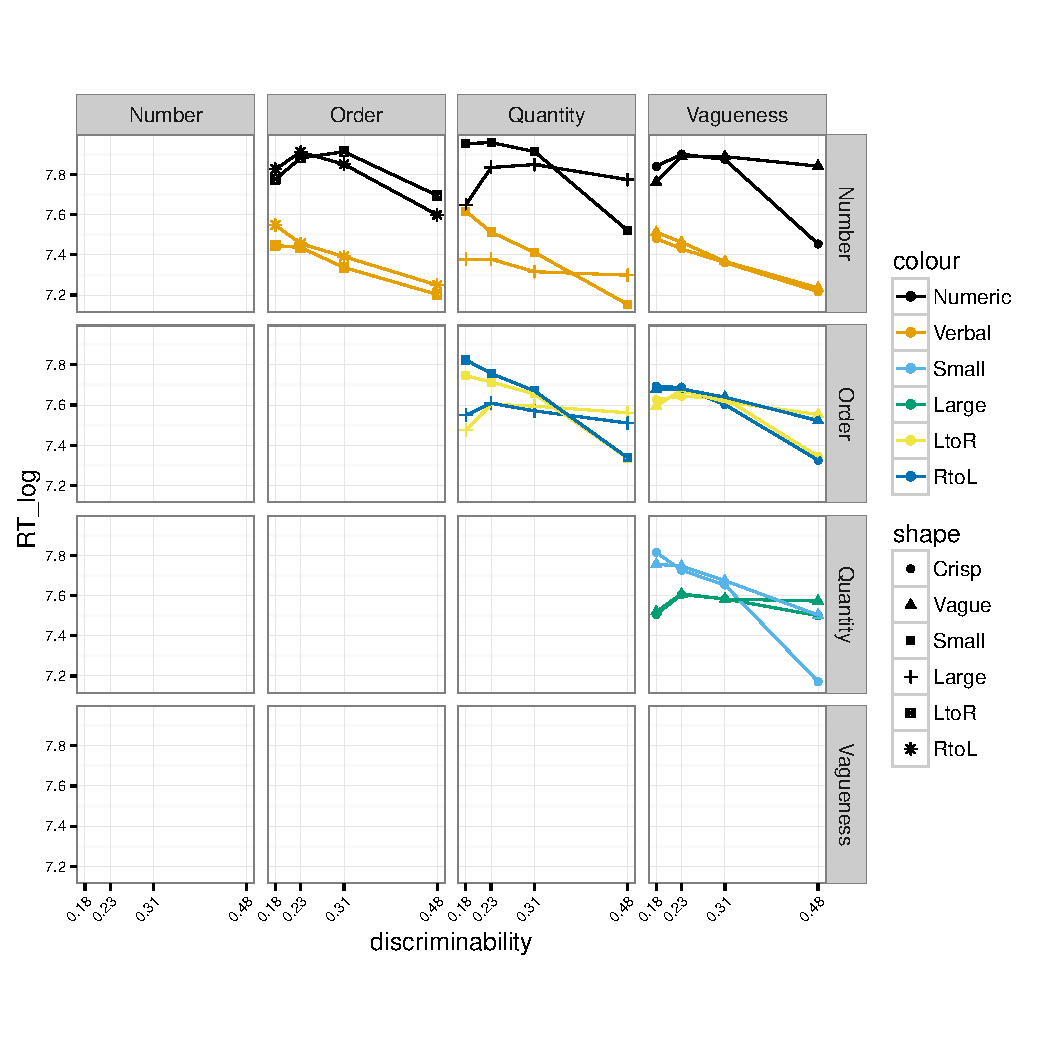
\includegraphics[width=\maxwidth]{figure/graphics-22way-1} 

}

\caption[2-way interactions over item ratios]{2-way interactions over item ratios}\label{fig:22way}
\end{figure}


\end{knitrout}

\clearpage

\begin{knitrout}\scriptsize
\definecolor{shadecolor}{rgb}{0.969, 0.969, 0.969}\color{fgcolor}\begin{figure}[hbtp]

{\centering 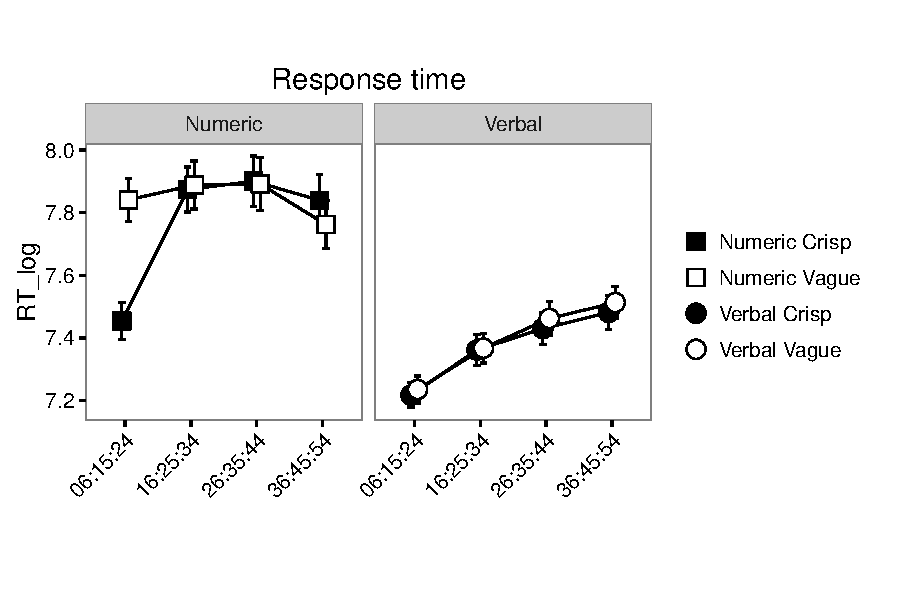
\includegraphics[width=\maxwidth]{figure/graphics-plotInt1-1} 

}

\caption[vagueness by number interaction over items]{vagueness by number interaction over items}\label{fig:plotInt1}
\end{figure}


\end{knitrout}

\clearpage

\begin{knitrout}\scriptsize
\definecolor{shadecolor}{rgb}{0.969, 0.969, 0.969}\color{fgcolor}\begin{figure}[hbtp]

{\centering 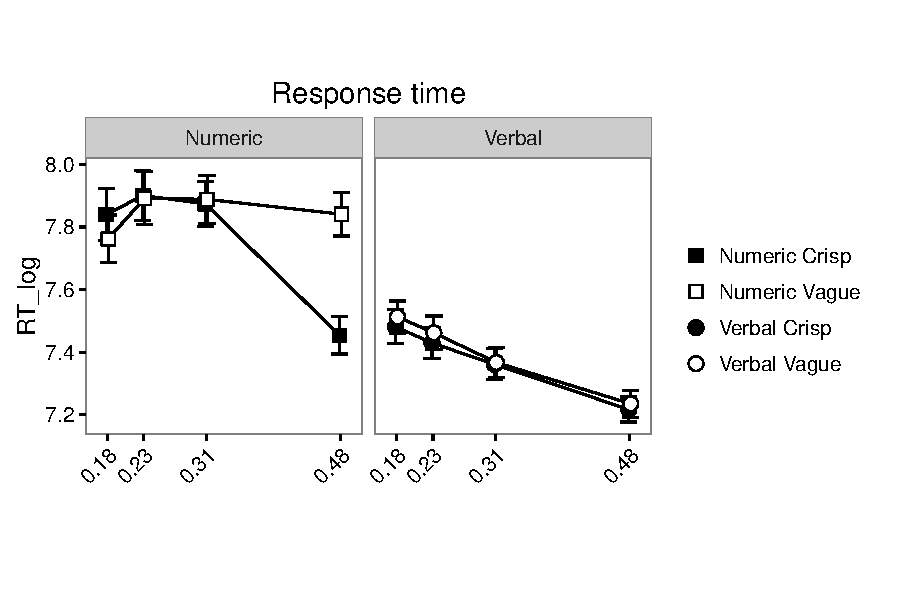
\includegraphics[width=\maxwidth]{figure/graphics-plotInt2-1} 

}

\caption[vagueness by number interaction over item ratios]{vagueness by number interaction over item ratios}\label{fig:plotInt2}
\end{figure}


\end{knitrout}

\clearpage

\begin{knitrout}\scriptsize
\definecolor{shadecolor}{rgb}{0.969, 0.969, 0.969}\color{fgcolor}\begin{figure}[hbtp]

{\centering 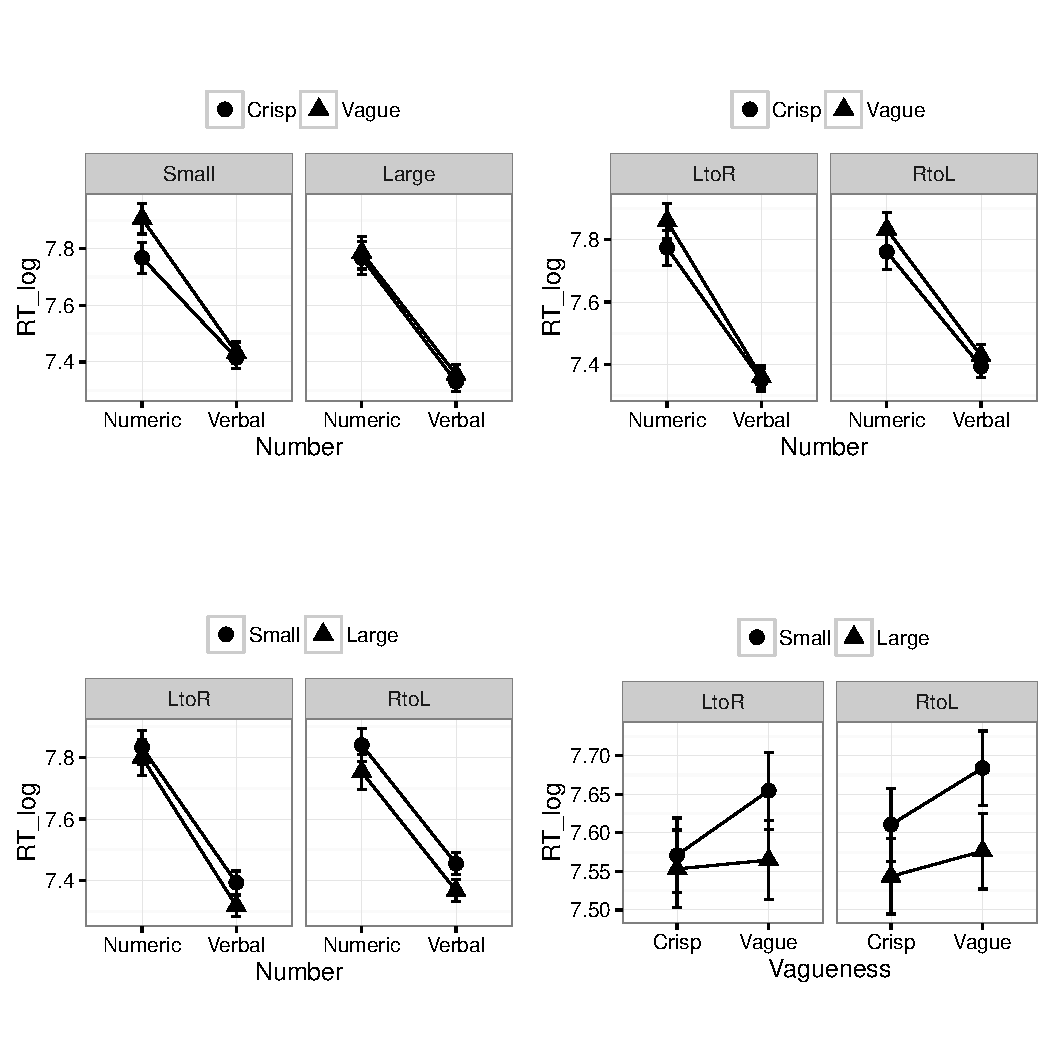
\includegraphics[width=\maxwidth]{figure/graphics-plot3way-1} 

}

\caption[3 way interactions]{3 way interactions}\label{fig:plot3way}
\end{figure}


\end{knitrout}

\clearpage

\begin{knitrout}\scriptsize
\definecolor{shadecolor}{rgb}{0.969, 0.969, 0.969}\color{fgcolor}\begin{figure}[hbtp]

{\centering 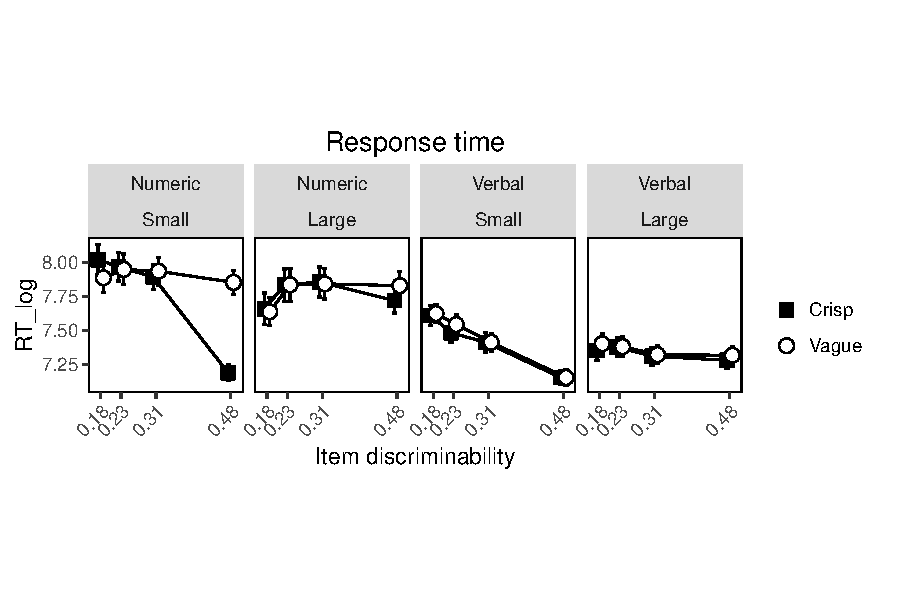
\includegraphics[width=\maxwidth]{figure/graphics-vnitems-1} 

}

\caption[Plot vagueness by number by quantity over item ratios]{Plot vagueness by number by quantity over item ratios.}\label{fig:vnitems}
\end{figure}


\end{knitrout}

\clearpage

\begin{knitrout}\scriptsize
\definecolor{shadecolor}{rgb}{0.969, 0.969, 0.969}\color{fgcolor}\begin{figure}[hbtp]

{\centering 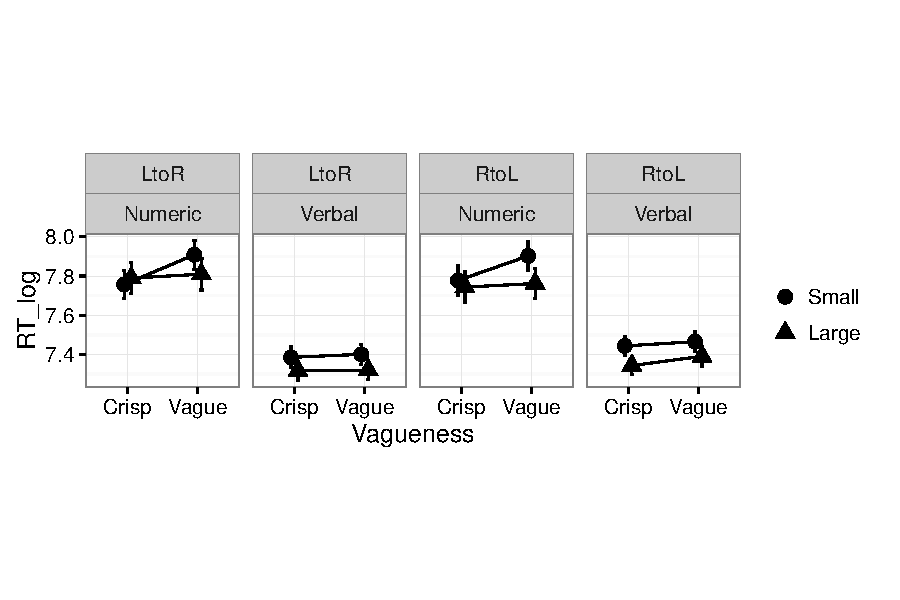
\includegraphics[width=\maxwidth]{figure/graphics-4way-1} 

}

\caption[4 way interaction]{4 way interaction}\label{fig:4way}
\end{figure}


\end{knitrout}

\clearpage

\begin{knitrout}\scriptsize
\definecolor{shadecolor}{rgb}{0.969, 0.969, 0.969}\color{fgcolor}\begin{figure}[hbtp]

{\centering 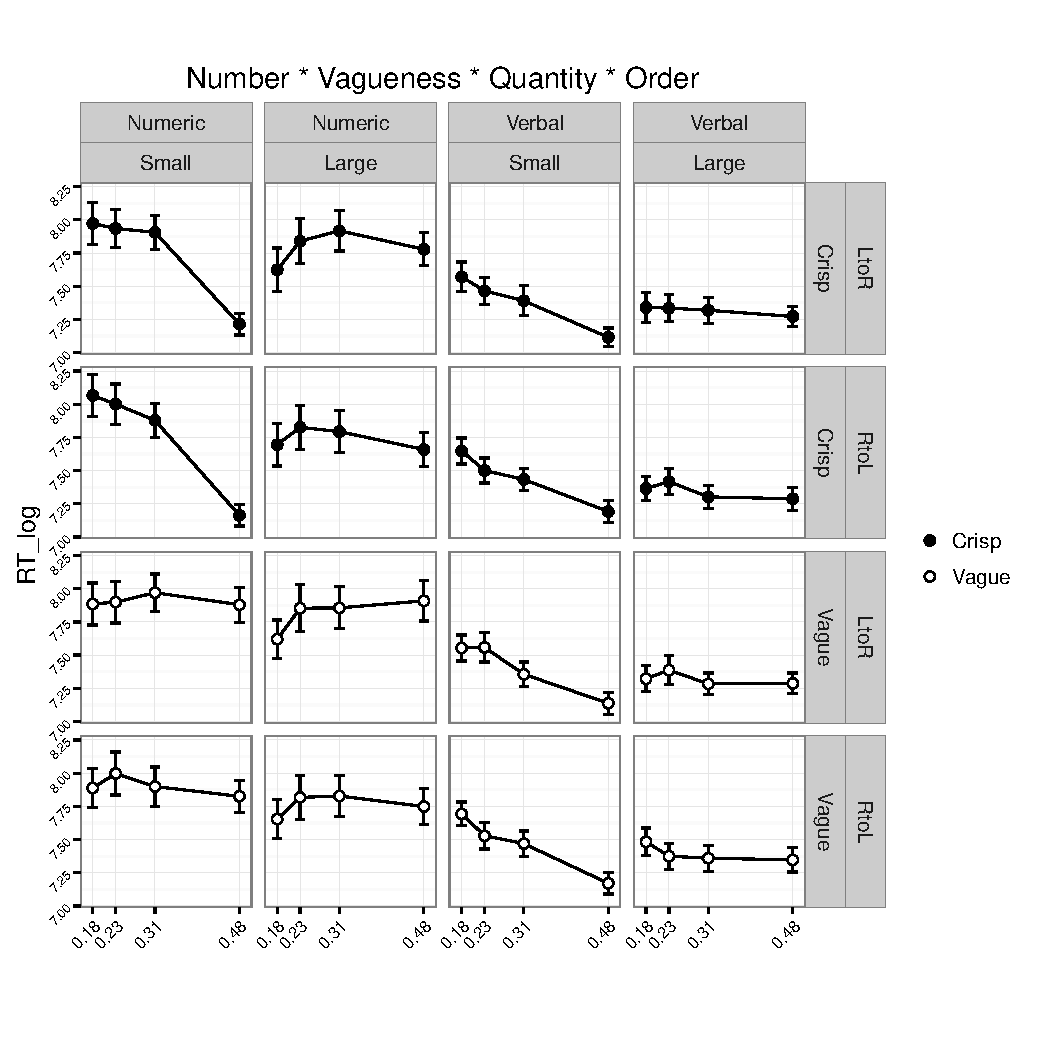
\includegraphics[width=\maxwidth]{figure/graphics-4waysplit-1} 

}

\caption[4 way interaction split over item discriminability]{4 way interaction split over item discriminability}\label{fig:4waysplit}
\end{figure}


\end{knitrout}

\clearpage
\section{Lmer model}

\begin{knitrout}\scriptsize
\definecolor{shadecolor}{rgb}{0.969, 0.969, 0.969}\color{fgcolor}\begin{kframe}
\begin{alltt}
\hlkwd{load}\hlstd{(}\hlstr{"data_processed.Rda"}\hlstd{)}
\end{alltt}
\end{kframe}
\end{knitrout}

\begin{knitrout}\scriptsize
\definecolor{shadecolor}{rgb}{0.969, 0.969, 0.969}\color{fgcolor}\begin{kframe}
\begin{alltt}
\hlstd{v5} \hlkwb{<-} \hlstd{lme4}\hlopt{::}\hlkwd{lmer}\hlstd{(}\hlkwc{data}\hlstd{=dd,}
                 \hlstd{RT_log} \hlopt{~}
                   \hlstd{c_Vag} \hlopt{+} \hlstd{c_Num} \hlopt{+} \hlstd{c_Qty} \hlopt{+} \hlstd{c_Ord} \hlopt{+}
                   \hlstd{c_Num}\hlopt{:}\hlstd{c_Vag}\hlopt{:}\hlstd{c_Qty} \hlopt{+}
                   \hlstd{discriminability} \hlopt{+}
                   \hlstd{s_Trl} \hlopt{+}
                   \hlstd{RTprev_log} \hlopt{+}
                   \hlstd{nchar_instr} \hlopt{+}
                   \hlstd{(}\hlnum{1}\hlopt{+}\hlstd{c_Vag} \hlopt{+} \hlstd{c_Num} \hlopt{+} \hlstd{c_Qty} \hlopt{+} \hlstd{c_Ord}\hlopt{|}\hlstd{Subject))}
\end{alltt}
\end{kframe}
\end{knitrout}

% latex table generated in R 3.3.1 by xtable 1.8-2 package
% Fri Aug 12 22:28:46 2016
\begin{table}[htbp]
\begingroup\small
\begin{tabular}{rrrr}
  \hline
 & Estimate & Std. Error & t value \\ 
  \hline
(Intercept) & 7.17 & 0.12 & 58.67 \\ 
  c\_Vag & 0.06 & 0.01 & 4.39 \\ 
  c\_Num & -0.43 & 0.08 & -5.77 \\ 
  c\_Qty & -0.07 & 0.02 & -3.45 \\ 
  c\_Ord & 0.02 & 0.01 & 1.33 \\ 
  discriminability & -0.77 & 0.05 & -15.66 \\ 
  s\_Trl & -0.11 & 0.01 & -18.42 \\ 
  RTprev\_log & 0.06 & 0.01 & 6.24 \\ 
  nchar\_instr & 0.01 & 0.00 & 3.13 \\ 
  c\_Vag:c\_Num:c\_Qty & 0.10 & 0.05 & 2.28 \\ 
   \hline
\end{tabular}
\endgroup
\caption{xtable v5} 
\end{table}


\begin{knitrout}\scriptsize
\definecolor{shadecolor}{rgb}{0.969, 0.969, 0.969}\color{fgcolor}\begin{kframe}
\begin{verbatim}
R^2
[1] 0.533722
\end{verbatim}
\end{kframe}
\end{knitrout}

\clearpage 

\begin{knitrout}\scriptsize
\definecolor{shadecolor}{rgb}{0.969, 0.969, 0.969}\color{fgcolor}\begin{figure}[hbtp]

{\centering 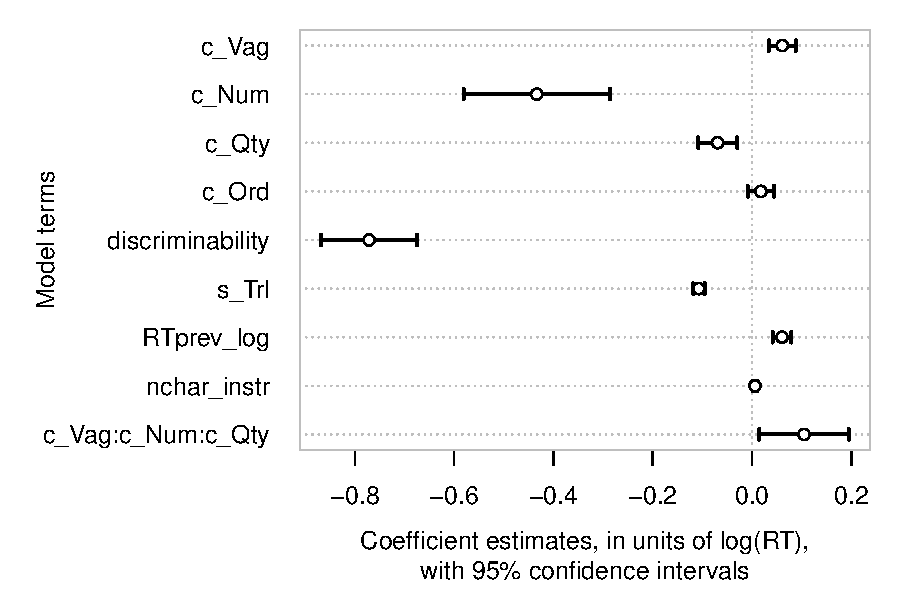
\includegraphics[width=\maxwidth]{figure/graphics-plotModelCoefsAndCis-1} 

}

\caption[Coefficient estimates and their (Wald) 95 per cent confidence intervals]{Coefficient estimates and their (Wald) 95 per cent confidence intervals}\label{fig:plotModelCoefsAndCis}
\end{figure}


\end{knitrout}


\clearpage 

\begin{knitrout}\scriptsize
\definecolor{shadecolor}{rgb}{0.969, 0.969, 0.969}\color{fgcolor}\begin{kframe}
\begin{alltt}
\hlkwd{par}\hlstd{(}\hlkwc{mfrow} \hlstd{=} \hlkwd{c}\hlstd{(}\hlnum{2}\hlstd{,} \hlnum{4}\hlstd{))}
\hlkwd{plotLMER.fnc}\hlstd{(v5)}
\end{alltt}
\begin{verbatim}
effect size (range) for  c_Vag is  0.03470056 
effect size (range) for  c_Num is  0.4073765 
effect size (range) for  c_Qty is  0.09530422 
effect size (range) for  c_Ord is  0.0179595 
effect size (range) for  discriminability is  0.2346348 
effect size (range) for  s_Trl is  0.369093 
effect size (range) for  RTprev_log is  0.2759499 
effect size (range) for  nchar_instr is  0.05477539 
\end{verbatim}
\end{kframe}\begin{figure}[hbtp]

{\centering 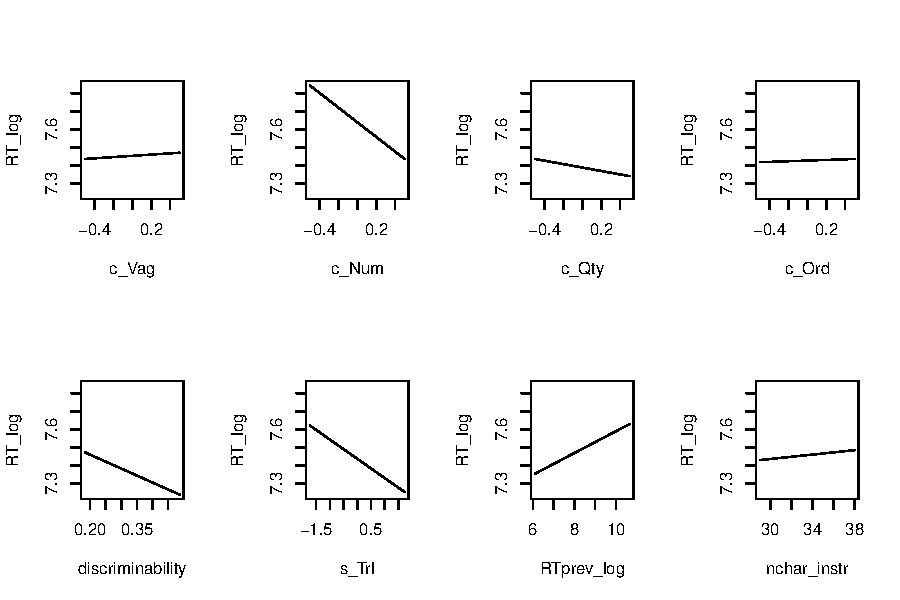
\includegraphics[width=\maxwidth]{figure/graphics-plotLMERfnc-1} 

}

\caption[plotMLERfnc]{plotMLERfnc}\label{fig:plotLMERfnc}
\end{figure}


\end{knitrout}

\clearpage

\begin{knitrout}\scriptsize
\definecolor{shadecolor}{rgb}{0.969, 0.969, 0.969}\color{fgcolor}\begin{figure}[hbtp]

{\centering 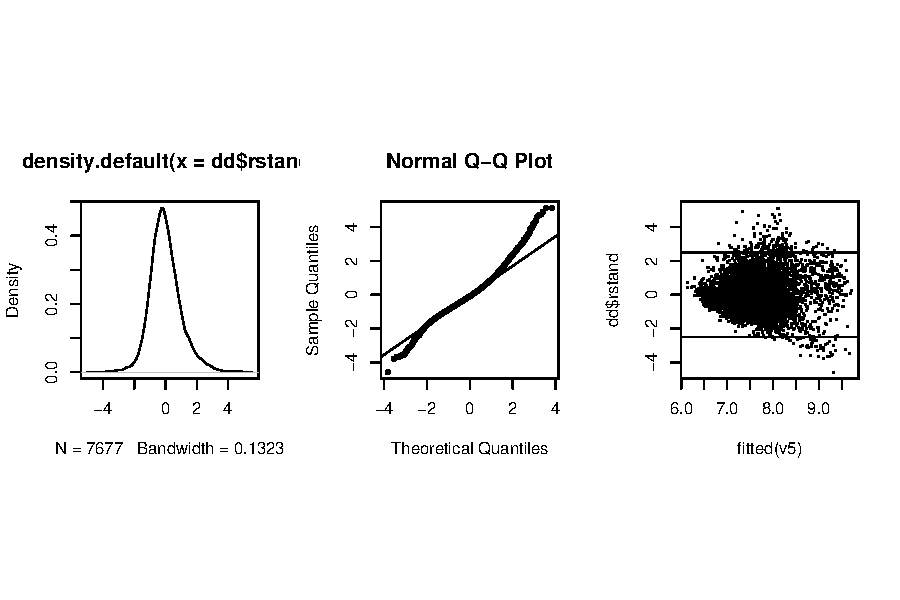
\includegraphics[width=\maxwidth]{figure/graphics-baayenPLots99-1} 

}

\caption[Baayen Model Criticism Plots]{Baayen Model Criticism Plots}\label{fig:baayenPLots99}
\end{figure}


\end{knitrout}

\clearpage

\section{lmerTest Version}

\begin{knitrout}\scriptsize
\definecolor{shadecolor}{rgb}{0.969, 0.969, 0.969}\color{fgcolor}\begin{kframe}
\begin{alltt}
\hlstd{v6} \hlkwb{<-} \hlstd{lmerTest}\hlopt{::}\hlkwd{lmer}\hlstd{(}\hlkwc{data} \hlstd{= dd, RT_log} \hlopt{~} \hlstd{c_Vag} \hlopt{+} \hlstd{c_Num} \hlopt{+} \hlstd{c_Qty} \hlopt{+} \hlstd{c_Ord} \hlopt{+} \hlstd{c_Num}\hlopt{:}\hlstd{c_Vag}\hlopt{:}\hlstd{c_Qty} \hlopt{+} \hlstd{discriminability} \hlopt{+}
    \hlstd{s_Trl} \hlopt{+} \hlstd{RTprev_log} \hlopt{+} \hlstd{nchar_instr} \hlopt{+} \hlstd{(}\hlnum{1} \hlopt{+} \hlstd{c_Vag} \hlopt{+} \hlstd{c_Num} \hlopt{+} \hlstd{c_Qty} \hlopt{+} \hlstd{c_Ord} \hlopt{|} \hlstd{Subject))}
\end{alltt}
\end{kframe}
\end{knitrout}

\begin{knitrout}\scriptsize
\definecolor{shadecolor}{rgb}{0.969, 0.969, 0.969}\color{fgcolor}\begin{kframe}
\begin{alltt}
\hlkwd{summary}\hlstd{(v6)}
\end{alltt}
\begin{verbatim}
Linear mixed model fit by REML t-tests use Satterthwaite approximations to degrees of freedom [
lmerMod]
Formula: RT_log ~ c_Vag + c_Num + c_Qty + c_Ord + c_Num:c_Vag:c_Qty +  
    discriminability + s_Trl + RTprev_log + nchar_instr + (1 +  
    c_Vag + c_Num + c_Qty + c_Ord | Subject)
   Data: dd

REML criterion at convergence: 11474.8

Scaled residuals: 
    Min      1Q  Median      3Q     Max 
-4.5470 -0.6351 -0.0955  0.5372  5.0914 

Random effects:
 Groups   Name        Variance Std.Dev. Corr                   
 Subject  (Intercept) 0.153949 0.39236                         
          c_Vag       0.001546 0.03932   0.69                  
          c_Num       0.165314 0.40659  -0.67 -0.64            
          c_Qty       0.008148 0.09027   0.16  0.26 -0.34      
          c_Ord       0.001559 0.03949  -0.13  0.02 -0.39 -0.52
 Residual             0.249734 0.49973                         
Number of obs: 7677, groups:  Subject, 30

Fixed effects:
                    Estimate Std. Error         df t value Pr(>|t|)    
(Intercept)        7.172e+00  1.222e-01  2.370e+02  58.671  < 2e-16 ***
c_Vag              6.094e-02  1.387e-02  3.300e+01   4.393 0.000112 ***
c_Num             -4.336e-01  7.515e-02  2.900e+01  -5.770 2.97e-06 ***
c_Qty             -6.907e-02  2.005e-02  2.900e+01  -3.445 0.001743 ** 
c_Ord              1.796e-02  1.350e-02  5.100e+01   1.331 0.189164    
discriminability  -7.714e-01  4.927e-02  7.551e+03 -15.658  < 2e-16 ***
s_Trl             -1.070e-01  5.807e-03  7.558e+03 -18.421  < 2e-16 ***
RTprev_log         6.047e-02  9.692e-03  7.594e+03   6.239 4.63e-10 ***
nchar_instr        6.086e-03  1.944e-03  7.551e+03   3.131 0.001749 ** 
c_Vag:c_Num:c_Qty  1.049e-01  4.607e-02  7.551e+03   2.278 0.022742 *  
---
Signif. codes:  0 '***' 0.001 '**' 0.01 '*' 0.05 '.' 0.1 ' ' 1

Correlation of Fixed Effects:
            (Intr) c_Vag  c_Num  c_Qty  c_Ord  dscrmn s_Trl  RTprv_ nchr_n
c_Vag        0.083                                                        
c_Num       -0.369 -0.337                                                 
c_Qty        0.069  0.117 -0.278                                          
c_Ord       -0.052  0.007 -0.206 -0.228                                   
discrmnblty -0.140  0.004 -0.001  0.000  0.001                            
s_Trl       -0.114  0.003 -0.001 -0.002  0.006  0.017                     
RTprev_log  -0.607  0.006 -0.004 -0.003  0.019  0.015  0.185              
nchar_instr -0.524  0.237 -0.034  0.018  0.000  0.017  0.000  0.006       
c_Vg:c_N:_Q  0.073 -0.033  0.005 -0.003  0.000 -0.002 -0.001 -0.002 -0.138
\end{verbatim}
\end{kframe}
\end{knitrout}

\clearpage
\section{Borderline responses}

\begin{knitrout}\scriptsize
\definecolor{shadecolor}{rgb}{0.969, 0.969, 0.969}\color{fgcolor}

{\centering 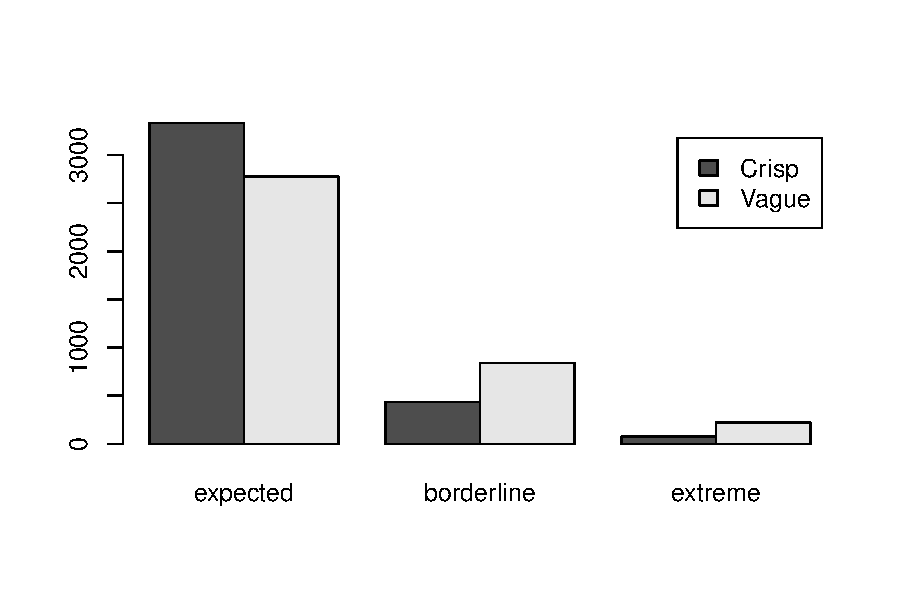
\includegraphics[width=\maxwidth]{figure/graphics-barplotBorderline-1} 

}



\end{knitrout}

% latex table generated in R 3.3.1 by xtable 1.8-2 package
% Fri Aug 12 22:28:47 2016
\begin{table}[htbp]
\centering
\begingroup\small
\begin{tabular}{rrr}
  \hline
 & Crisp & Vague \\ 
  \hline
expected & 3332 & 2776 \\ 
  borderline & 433 & 841 \\ 
  extreme &  75 & 220 \\ 
   \hline
\end{tabular}
\endgroup
\caption{Borderline cases counts} 
\end{table}


\end{document}
